\ylDisplay{Kaater} % Ülesande nimi
{Jaan Kalda} % Autor
{lõppvoor} % Voor
{2009} % Aasta
{G 8} % Ülesande nr.
{8} % Raskustase
{
% Teema: Kinemaatika
\ifStatement
Mootorpaat sõidab jõe ühelt kaldalt punktist A teisele kaldale punkti B. Paadi kiirus on $u=\SI{7}{m/s}$.\\
\osa Joonisel on näidatud paadi tekitatud veelained. Milline on jõe voolukiirus?\\
\osa On teada, et kui vee sügavus on $h$, siis lained levivad kiirusega $w=\sqrt{gh}$, kus $g$ on vabalangemise kiirendus.
Kui sügav on jõgi?

\begin{center}
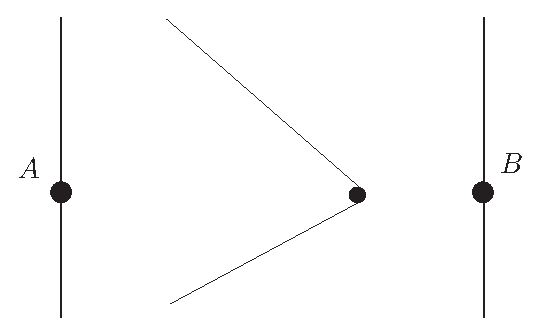
\includegraphics[width=0.55\linewidth]{2009-v3g-08-paat.eps}
\end{center}
\fi


\ifHint
Olukorda on mugavam vaadelda veega seotud taustsüsteemis, sest siis liiguvad lained paadi trajektoori suhtes sümmeetriliselt (lainefrondid on paadi varasematest asukohtadest eemalduvad ringid).
\fi


\ifSolution
\osa
Veega seotud taustsüsteemis liiguvad lained paadi trajektoori suhtes sümmeetriliselt. Seega, veega seotud taustsüsteemis on
paadi trajektoor lainetest moodustatud nurga poolitaja. Paadi kiirusest $\vec u$, jõe voolukiirusest $\vec v$ ja paadi kiirusest maa suhtes moodustub kiiruste kolmnurk, vt joonis.
Jooniselt mõõdame selle kolmnurga teravama nurga siinuse, $\sin \alpha =v/u=\num{0.26}$, millest $v=\SI{1.8}{m/s}$.

\begin{center}
	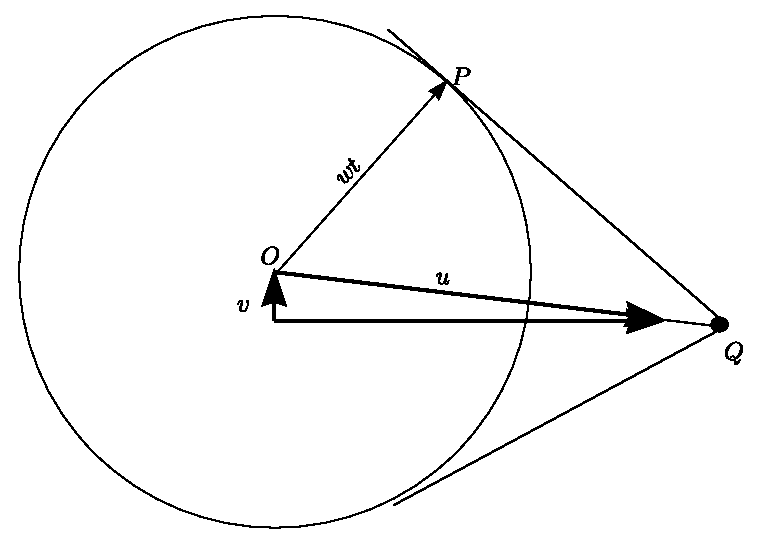
\includegraphics[width=0.8\linewidth]{2009-v3g-08-paatlah.eps}
\end{center}

\osa
Kui paat tekitas teatud punktis häirituse, siis levis see ajaga $t$ kaugusele $wt$ (nähtavaks paadilaineks on selliste ringide mähisjoon),
paat aga liikus kaugusele $ut$. Seega leiame jooniselt pikkuste suhte abil $w/u=|OP|/|OQ|=\num{0.64}$, millest $w=\SI{4.5}{m/s}$. Järelikult on vee sügavus
$h=w^2/g=2\,$m.
\fi
}